\section{Results}

\subsection{Single-shot model performance}
% How did we come up with linear models:
% 	- compare performance of all models by "recall"
% 	- compare time with the actual docking time
% 	- test effects of normalization

In order to select most promising models for active-learning iterations, we first compared them on a single batch. As shown in figure \ref{fig:fig_4}, both on retrospective data \cite{ultralarge_docking_first} and data present in this paper, different models show comparable recall, that also becomes more reproducible with the increase of the train size dataset. Expectedly, more complex models such as RandomForestRegressor show superior performance compared to more simple models, albeit at the expense of the significantly increased training and inference time (up to 3 orders of magnitude). Note that here the train dataset size and inference size are related as 4:1 due to 5-fold validation (see \ref{subsec:prediction}). 

Paragraph about docking-as-predictor performance in single-shot.

Paragraph about effect of normalization

\begin{figure}[h]
% Fig 4: selection of the best single model
% 	- A: model performances
% 	- B: model timing
% 	- C: time vs performance distribution + actual docking time cutoff
\centering
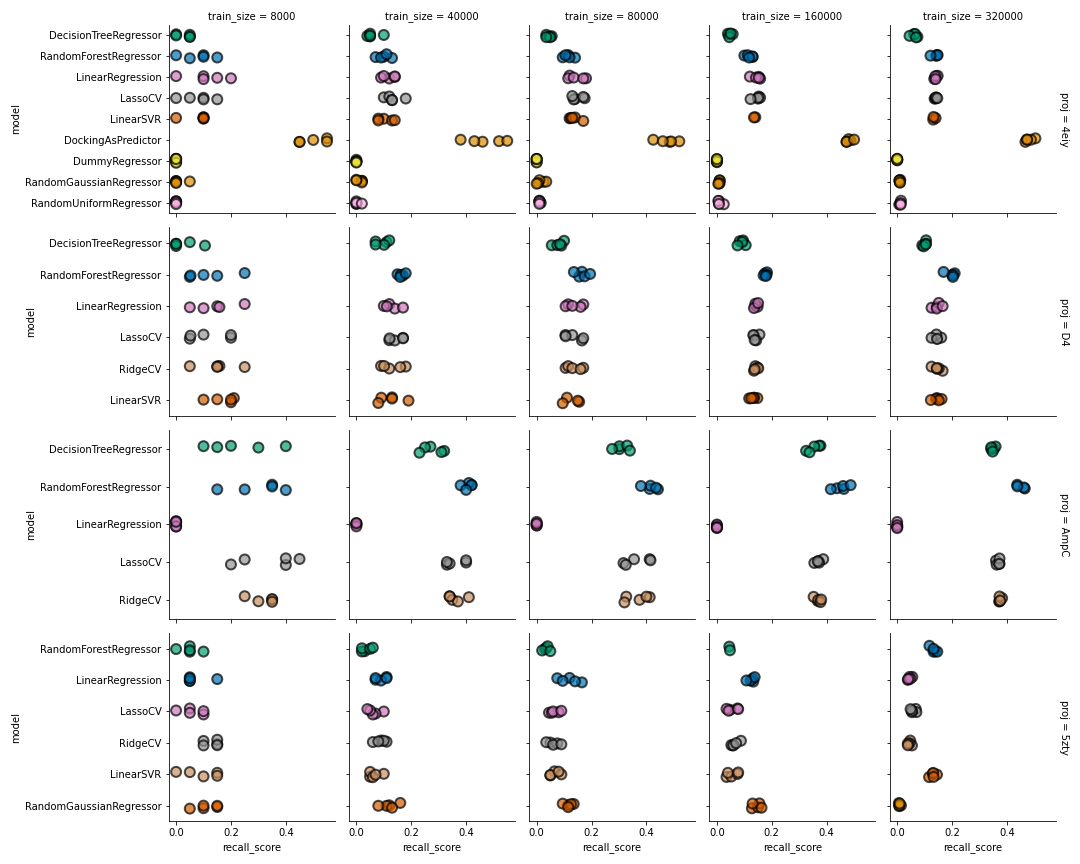
\includegraphics[width=0.8\textwidth]{figures/Figure_4.png}
% 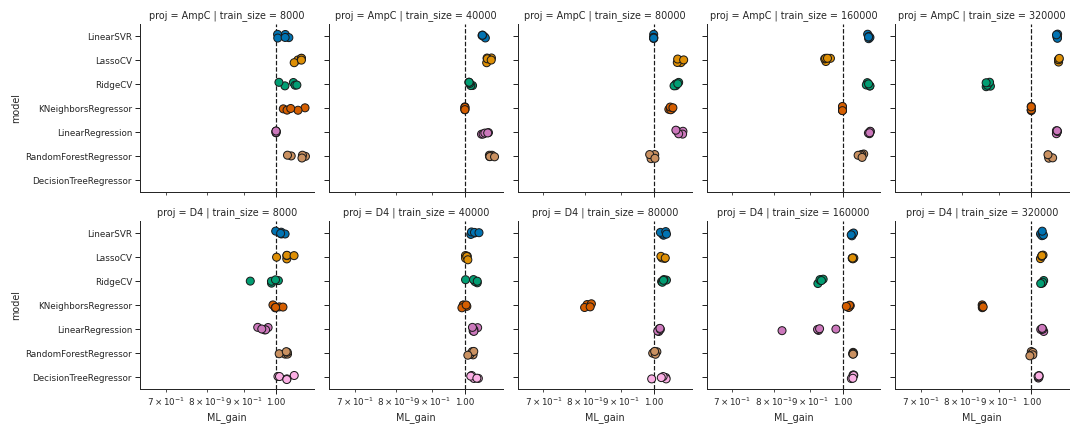
\includegraphics[width=0.8\textwidth]{figures/Figure_4_gain.png}
\caption{Model performance versus training and inference time (in logarithmic scale)}
\label{fig:fig_4}
\end{figure}

\subsection{Optimization of active learning regime}
% How did we come up with iterations scheme:
% 	- compared different train sizes
% 	- compared different regimes (add/noadd)
% 	- compared different ensembling methods
% 	- compare with "docking-as-predictor"

\begin{figure}[h]
% Fig 5: fine-tuning metaparameters of "iterations" 
% 	- batch size effect on the iterations performance
% 	- add/noadd & different ranking schemes effect
% 	- comparison  of the best model with with docking-as-predictor
% 	- TODO: comparison with the really best single model
\centering
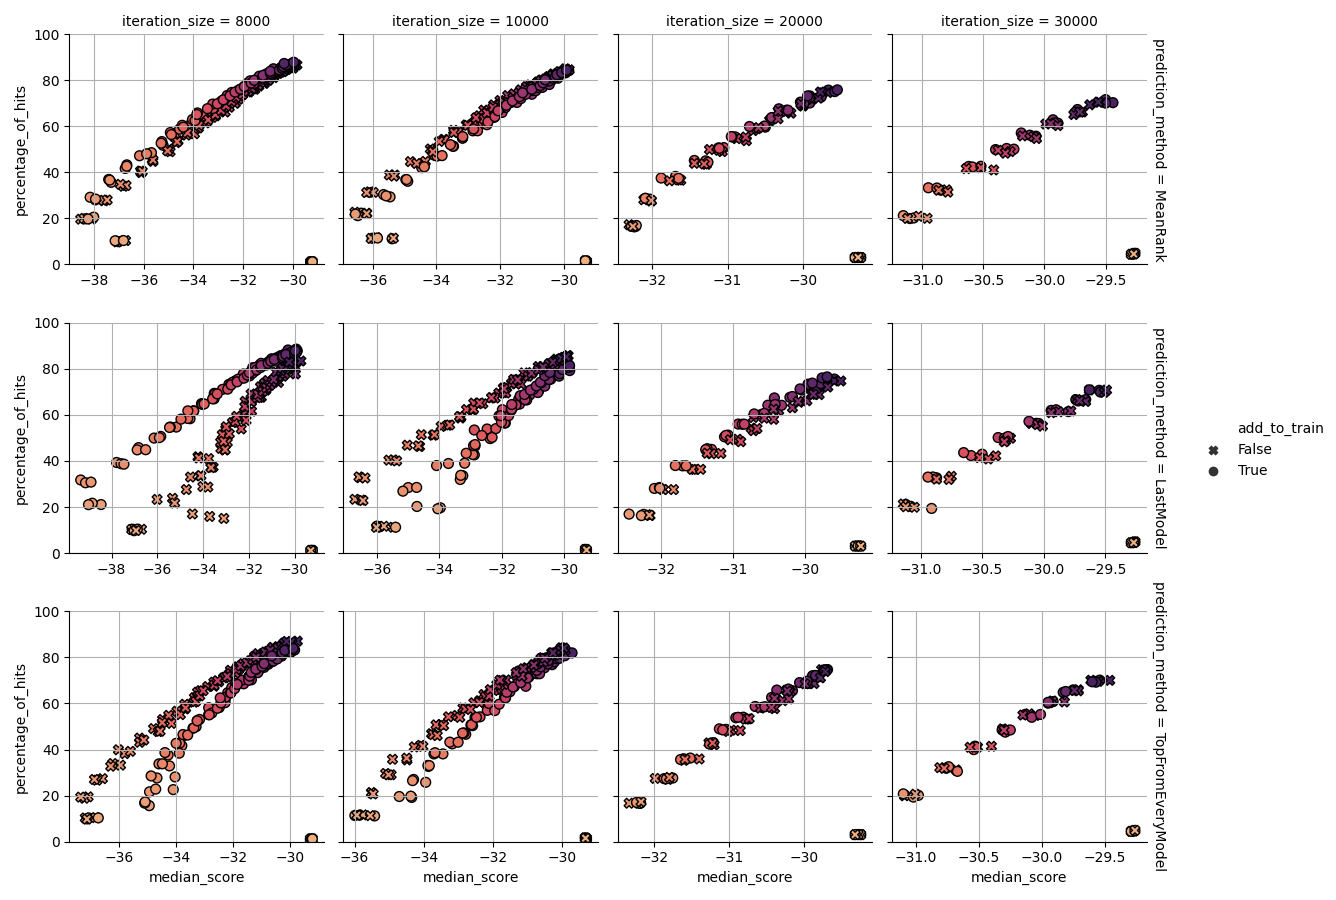
\includegraphics[width=0.8\textwidth]{figures/Figure_3.png}
\caption{Model performance in active learning regime}
\label{fig:fig_3}
\end{figure}

